% Options for packages loaded elsewhere
\PassOptionsToPackage{unicode}{hyperref}
\PassOptionsToPackage{hyphens}{url}
%
\documentclass[
]{book}
\title{Similitud de Comunidades biológicas}
\author{Carlos Iván Espinosa}
\date{Enero 2022}

\usepackage{amsmath,amssymb}
\usepackage{lmodern}
\usepackage{iftex}
\ifPDFTeX
  \usepackage[T1]{fontenc}
  \usepackage[utf8]{inputenc}
  \usepackage{textcomp} % provide euro and other symbols
\else % if luatex or xetex
  \usepackage{unicode-math}
  \defaultfontfeatures{Scale=MatchLowercase}
  \defaultfontfeatures[\rmfamily]{Ligatures=TeX,Scale=1}
\fi
% Use upquote if available, for straight quotes in verbatim environments
\IfFileExists{upquote.sty}{\usepackage{upquote}}{}
\IfFileExists{microtype.sty}{% use microtype if available
  \usepackage[]{microtype}
  \UseMicrotypeSet[protrusion]{basicmath} % disable protrusion for tt fonts
}{}
\makeatletter
\@ifundefined{KOMAClassName}{% if non-KOMA class
  \IfFileExists{parskip.sty}{%
    \usepackage{parskip}
  }{% else
    \setlength{\parindent}{0pt}
    \setlength{\parskip}{6pt plus 2pt minus 1pt}}
}{% if KOMA class
  \KOMAoptions{parskip=half}}
\makeatother
\usepackage{xcolor}
\IfFileExists{xurl.sty}{\usepackage{xurl}}{} % add URL line breaks if available
\IfFileExists{bookmark.sty}{\usepackage{bookmark}}{\usepackage{hyperref}}
\hypersetup{
  pdftitle={Similitud de Comunidades biológicas},
  pdfauthor={Carlos Iván Espinosa},
  hidelinks,
  pdfcreator={LaTeX via pandoc}}
\urlstyle{same} % disable monospaced font for URLs
\usepackage{longtable,booktabs,array}
\usepackage{calc} % for calculating minipage widths
% Correct order of tables after \paragraph or \subparagraph
\usepackage{etoolbox}
\makeatletter
\patchcmd\longtable{\par}{\if@noskipsec\mbox{}\fi\par}{}{}
\makeatother
% Allow footnotes in longtable head/foot
\IfFileExists{footnotehyper.sty}{\usepackage{footnotehyper}}{\usepackage{footnote}}
\makesavenoteenv{longtable}
\usepackage{graphicx}
\makeatletter
\def\maxwidth{\ifdim\Gin@nat@width>\linewidth\linewidth\else\Gin@nat@width\fi}
\def\maxheight{\ifdim\Gin@nat@height>\textheight\textheight\else\Gin@nat@height\fi}
\makeatother
% Scale images if necessary, so that they will not overflow the page
% margins by default, and it is still possible to overwrite the defaults
% using explicit options in \includegraphics[width, height, ...]{}
\setkeys{Gin}{width=\maxwidth,height=\maxheight,keepaspectratio}
% Set default figure placement to htbp
\makeatletter
\def\fps@figure{htbp}
\makeatother
\setlength{\emergencystretch}{3em} % prevent overfull lines
\providecommand{\tightlist}{%
  \setlength{\itemsep}{0pt}\setlength{\parskip}{0pt}}
\setcounter{secnumdepth}{5}
\usepackage{booktabs}
\ifLuaTeX
  \usepackage{selnolig}  % disable illegal ligatures
\fi
\usepackage[]{natbib}
\bibliographystyle{apalike}

\begin{document}
\maketitle

{
\setcounter{tocdepth}{1}
\tableofcontents
}
\hypertarget{prefacio}{%
\chapter*{Prefacio}\label{prefacio}}
\addcontentsline{toc}{chapter}{Prefacio}

\begin{center}\rule{0.5\linewidth}{0.5pt}\end{center}

La comunidad biológica se refiere a una agrupación de poblaciones de especies que se presentan juntas en el espacio y el tiempo (Begon et al.~1999). Este concepto plantea que las comunidades tienen unos límites espaciales y temporales. Estos límites están dados por la distribución de las poblaciones a lo largo de un gradiente espacial o temporal. De esta forma los cambios en abundancia de las especies a lo largo de gradientes espaciales o temporales generan la zonación y la sucesión respectivamente.

La identificación de formaciones biológicas en el espacio (\textbf{zonación}), o las etapas seriales a lo largo del tiempo (\textbf{sucesión}), implica qué tenemos la capacidad de establecer en qué momento una comunidad cambia. Parece una tarea sencilla, pero realmente no lo es, ¿cuánto debería cambiar una comunidad para poder hablar de etapas seriales o zonas distintas? y ¿cómo podemos calcular ese cambio? Una de las formas de responder estas preguntas puede ser intentar cuantificar las similitudes entre localidades.

\hypertarget{objetivos}{%
\chapter*{Objetivos}\label{objetivos}}
\addcontentsline{toc}{chapter}{Objetivos}

\begin{center}\rule{0.5\linewidth}{0.5pt}\end{center}

En este ejercicio mostramos las bases del cálculo de similitud y distancia entre comunidades, el cual se convierte en la base de los análisis multivariantes de la comunidad.

Específicamente nos interesa;

\begin{itemize}
\tightlist
\item
  Comprender las bases teóricas para el cálculo de similitudes y distancias en la comunidad entre localidades.
\item
  Desarrollar mediciones de similitud entre localidades e interpretar los resultados.
\end{itemize}

\begin{figure}
\centering
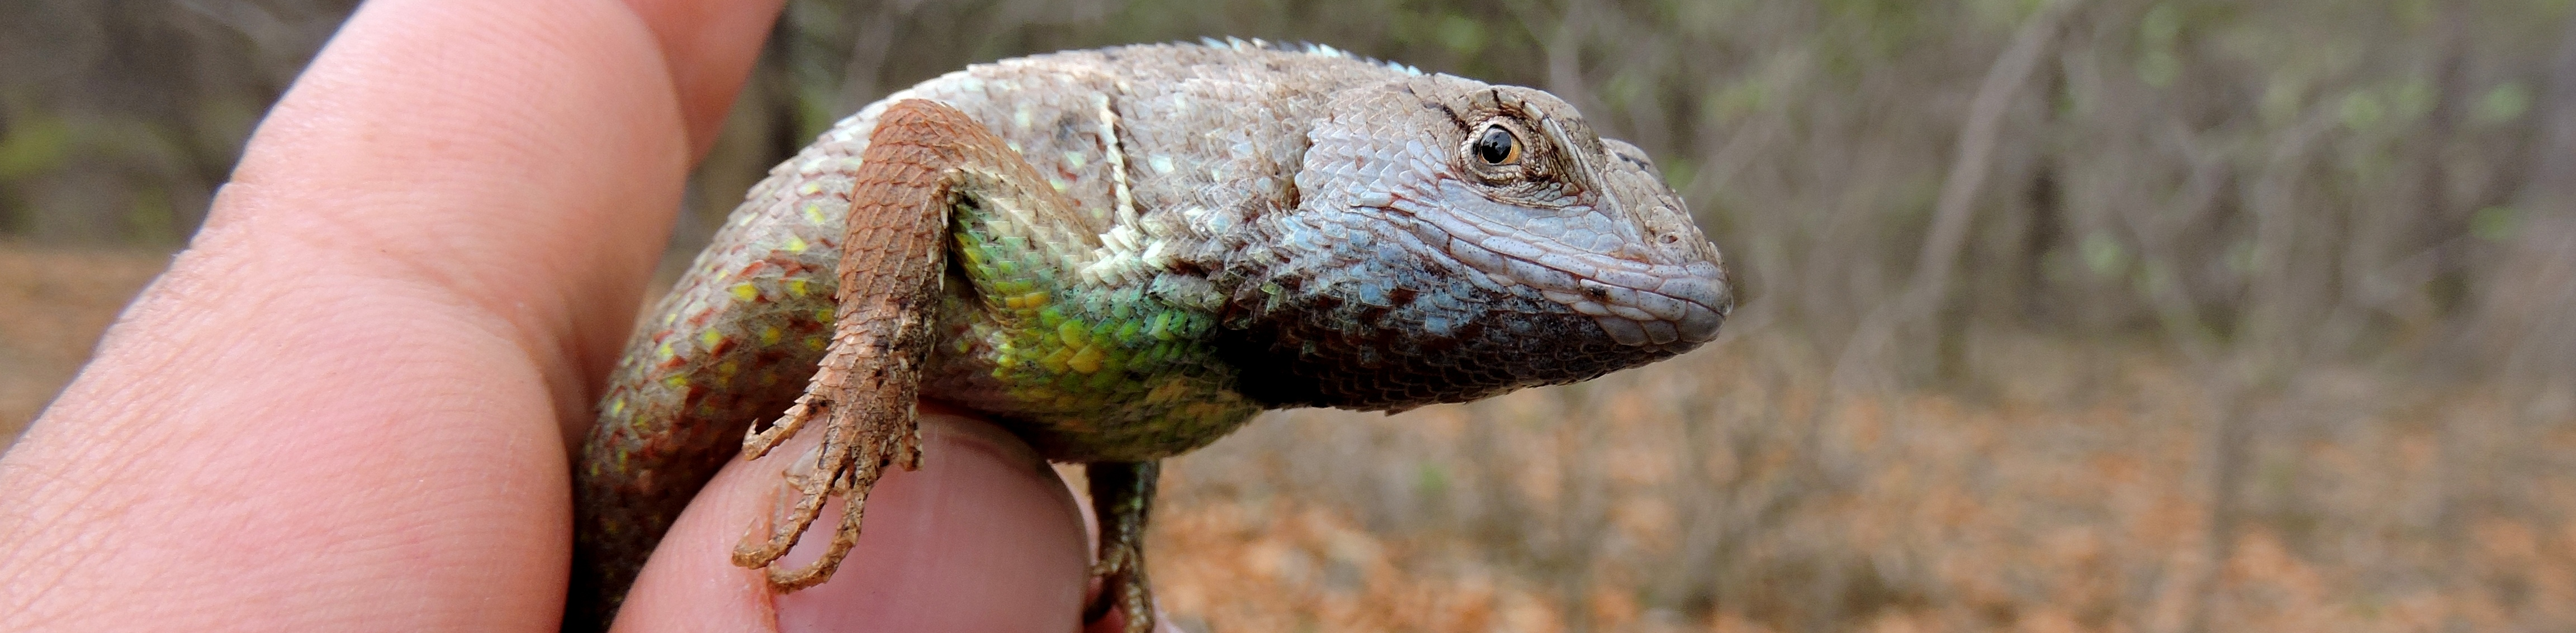
\includegraphics{lagar.jpg}
\caption{\emph{Stenocercus iridicens}}
\end{figure}

\hypertarget{introducciuxf3n}{%
\chapter{Introducción}\label{introducciuxf3n}}

Placeholder

\hypertarget{uxedndices-cualitativos}{%
\section{Índices cualitativos}\label{uxedndices-cualitativos}}

\hypertarget{uxedndices-cuantitativos}{%
\section{Índices cuantitativos}\label{uxedndices-cuantitativos}}

\hypertarget{distancia-euclidiana}{%
\section{Distancia Euclidiana}\label{distancia-euclidiana}}

\hypertarget{efecto-de-doble-ceros-y-abundancia}{%
\subsection{Efecto de doble-ceros y abundancia}\label{efecto-de-doble-ceros-y-abundancia}}

\hypertarget{efecto-de-la-abundancia}{%
\subsection{Efecto de la abundancia}\label{efecto-de-la-abundancia}}

\hypertarget{distancia-bray-curtis}{%
\section{Distancia Bray-Curtis}\label{distancia-bray-curtis}}

\hypertarget{transformaciuxf3n-de-datos}{%
\section{Transformación de datos}\label{transformaciuxf3n-de-datos}}

\hypertarget{estandarizaciuxf3n-de-los-datos}{%
\section{Estandarización de los datos}\label{estandarizaciuxf3n-de-los-datos}}

  \bibliography{packages.bib}

\end{document}
